\documentclass[12 pt]{amsart}
\usepackage{amsmath, amssymb, amsthm,amscd}
\usepackage{tkz-graph}
\usepackage{tikz}
\usepackage{tikz,fullpage}
\usetikzlibrary{positioning, quotes}
\usetikzlibrary{arrows,%
                petri,%
                topaths}%
\usetikzlibrary{graphs,quotes}
\usetikzlibrary{arrows,automata}
\usepackage[latin1]{inputenc}
\usepackage{tkz-berge}
\usepackage[position=top]{subfig}

\allowdisplaybreaks

\newcommand{\mathsym}[1]{{}}
\newcommand{\unicode}{{}}

\newtheorem{theorem}{Theorem}[section]
\newtheorem{lemma}[theorem]{Lemma}
\newtheorem{proposition}[theorem]{Proposition}
\newtheorem{corollary}[theorem]{Corollary}
\newtheorem{definition}[theorem]{Definition}
\newtheorem{construction}[theorem]{Construction}

\newcommand\T{\rule{0pt}{-1.0ex}}       % Top strut
\newcommand\B{\rule[0.5ex]{0pt}{0pt}} % Bottom strut

\newcommand{\smat}[4] {(\begin{smallmatrix} #1 & #2 \\ #3 & #4 \end{smallmatrix} )}
\newcommand{\mat}[4]  { \left(\begin{array}{cc} #1 & #2 \\ #3 & #4 \end{array} \right)}
\newcommand{\schar}[2] {( \begin{smallmatrix} #1 \\ #2 \end{smallmatrix})}

\newcommand{\op}[1]  { \operatorname{ #1 }}
\newcommand{\olbbH}[0]  { \overline{\mathbb{H}}}
\newcommand{\olbbQ}[0]  { \overline{\mathbb{Q}}}
\newcommand{\olG}[0]  { \overline{\Gamma}}
\newcommand{\bbH}[0]  { \mathbb{H}}
\newcommand{\bbC}[0]  { \mathbb{C}}
\newcommand{\bbZ}[0]  { \mathbb{Z}}
\newcommand{\bbF}[0]  { \mathbb{F}}
\newcommand{\bbQ}[0]  { \mathbb{Q}}
\newcommand{\bbR}[0]  { \mathbb{R}}
\newcommand{\gok}[0]  { \mathfrak{k}}
\newcommand{\goe}[0]  { \mathfrak{e}}
\newcommand{\goR}[0]  { \mathfrak{R}}

\newcommand{\om}[2] {\omega_{#1}^{#2}}

\usepackage{bbm}
\newcommand{\ee}[0] {\mathbbm{e}}
\newcommand{\ii}[0] {\mathbbm{i}}

%\newcommand{\ee}[0] {e}
%\newcommand{\ii}[0] {i}

\addtolength{\textwidth}{1.0in}
\addtolength{\hoffset}{-0.5in}
\addtolength{\textheight}{0.0in}
\addtolength{\voffset}{-0.0in}

\begin{document}
\title{fft}

\section{notation}

\begin{tabular}{l|l}
$\ii$ & $\sqrt{-1}$ \\
$\ee$ & $2.71\dots$ \\
$\pi$ & $3.14\dots$ \\
$\operatorname{EvalPoly}(a, \vec{x})$ & $\sum_{0 \le i < n} x_i a^i$, $\vec{x} = (x_0, \dots, x_{n-1})$\\
$\om{b}{a}$ & $\ee^{2 a \pi \ii / b}$ a $b^{\text{th}}$ root of unity\\
$\overline{i}^k$ & length $k$ bit-reversal of $i$. Only defined for $0 \le i < 2^k$\\
\end{tabular} 

\section{fft/ifft}

Unless the output of the fft is specifically needed to be in the usual order
\begin{equation*}
\left\{\operatorname{EvalPoly}(\om{2^k}{i}, \vec{x})\right\}_{0 \le i < 2^k}
\end{equation*}
there is no reason not to give the output in bit-reversed order
\begin{equation*}
\left\{\operatorname{EvalPoly}(\om{2^k}{\overline{i}^k}, \vec{x})\right\}_{0 \le i < 2^k}\text{.}
\end{equation*}
The reason being here is that the bit-reversed output is much simpler and faster because it
groups similar outputs close together. For example, $\operatorname{EvalPoly}(1, \vec{x})$ and
$\operatorname{EvalPoly}(-1, \vec{x})$ are very similar computationally and are right next to
each other in the bit-reversed output, but are very far apart in the usual order. Therefore,
we will restrict exclusively to bit-reversed outputs.


The usual sequence for calculating a length $16$ fft follows the columns below and ends with
the fft in the last column.
\begin{center}
\begin{tabular}{c|c|c|c|c}
$x_i$ & $y_i$ & $z_i$ & $w_i$ & $\operatorname{fft}(\vec{x})$\\
\hline
 $x_{0}$ &  $x_{0}+x_{8}$              & $y_{0}+y_{4}$              & $z_{0}+z_{2}$              & $w_{0} + w_{1}$\T\B\\
 $x_{1}$ &  $x_{1}+x_{9}$              & $y_{1}+y_{5}$              & $z_{1}+z_{3}$              & $(w_{0} - w_{1})$\T\B\\
 $x_{2}$ &  $x_{2}+x_{10}$             & $y_{2}+y_{6}$              & $(z_{0}-z_{2})\om{4}{0}$   & $w_{2} + w_{3}$\T\B\\
 $x_{3}$ &  $x_{3}+x_{11}$             & $y_{3}+y_{7}$              & $(z_{2}-z_{3})\om{4}{1}$   & $(w_{2} - w_{3})$\T\B\\
 $x_{4}$ &  $x_{4}+x_{12}$             & $(y_{0}-y_{4})\om{8}{0}$   & $z_{4}+z_{6}$              & $w_{4} + w_{5}$\T\B\\
 $x_{5}$ &  $x_{5}+x_{13}$             & $(y_{1}-y_{5})\om{8}{1}$   & $z_{5}+z_{7}$              & $(w_{4} - w_{5})$\T\B\\
 $x_{6}$ &  $x_{6}+x_{14}$             & $(y_{2}-y_{6})\om{8}{2}$   & $(z_{4}-z_{6})\om{4}{0}$   & $w_{6} + w_{7}$\T\B\\
 $x_{7}$ &  $x_{7}+x_{15}$             & $(y_{3}-y_{7})\om{8}{3}$   & $(z_{5}-z_{7})\om{4}{1}$   & $(w_{6} - w_{7})$\T\B\\
 $x_{8}$ &  $(x_{0}-x_{8})\om{16}{0}$  & $y_{8}+y_{12}$             & $z_{8}+z_{10}$             & $w_{8} + w_{9}$\T\B\\
 $x_{9}$ &  $(x_{1}-x_{9})\om{16}{1}$  & $y_{9}+y_{13}$             & $z_{9}+z_{11}$             & $(w_{8} - w_{9})$\T\B\\
$x_{10}$ &  $(x_{2}-x_{10})\om{16}{2}$ & $y_{10}+y_{14}$            & $(z_{8}-z_{10})\om{4}{0}$  & $w_{10} + w_{11}$\T\B\\
$x_{11}$ &  $(x_{3}-x_{11})\om{16}{3}$ & $y_{11}+y_{15}$            & $(z_{9}-z_{11})\om{4}{1}$  & $(w_{10} - w_{11})$\T\B\\
$x_{12}$ &  $(x_{4}-x_{12})\om{16}{4}$ & $(y_{8}-y_{12})\om{8}{0}$  & $z_{12}+z_{14}$            & $w_{12} + w_{13}$\T\B\\
$x_{13}$ &  $(x_{5}-x_{13})\om{16}{5}$ & $(y_{9}-y_{13})\om{8}{1}$  & $z_{13}+z_{15}$            & $(w_{12} - w_{13})$\T\B\\
$x_{14}$ &  $(x_{6}-x_{14})\om{16}{6}$ & $(y_{10}-y_{14})\om{8}{2}$ & $(z_{12}-z_{14})\om{4}{0}$ & $w_{14} + w_{15}$\T\B\\
$x_{15}$ &  $(x_{7}-x_{15})\om{16}{7}$ & $(y_{11}-y_{15})\om{8}{3}$ & $(z_{13}-z_{15})\om{4}{1}$ & $(w_{14} - w_{15})$\T\B\\
\end{tabular} 
\end{center}
One problem with this approach is that each column accesses many different
\emph{twiddle factors} $\omega_b^a$. In the case of a Sch\"onhage--Strassen fft where the base
ring is $\mathbb{Z}/(2^{m}+1)\mathbb{Z}$, this doesn't matter because each twiddle factor is a
power of two and implemented via bit shifts. In other cases, these twiddle factors have to be
either computed on the fly or precomputed and then retrieved from storage. In the case of precomputation,
we have to have in memory the table
\begin{equation*}
1,\om{2}{1}, 1,\om{4}{1}, 1, \om{8}{1}, \om{8}{2}, \om{8}{3}, 1, \om{16}{1}, \om{16}{2}, \om{16}{3}, \om{16}{4}, \om{16}{5}, \om{16}{6}, \om{16}{7}, 1, \dots
\end{equation*}
so that the columns can access this table sequentially. However, such a table is nice because
once it is extended to accomodate an fft of a certain length, it can be reused for all ffts of
smaller length.

By rearranging the twiddle factors as ($\omega = \omega_{16}$)

\begin{center}
\begin{tabular}{c|c|c|c|c}
$x_i$ & $y_i$ & $z_i$ & $w_i$ & $\operatorname{fft}(\vec{x})$\\
\hline
 $x_{0}$ &  $x_{0}+\om{}{0}x_{8}$  & $y_{0}+\om{}{0}y_{4}$    & $z_{0}+\om{}{0}z_{2}$    & $w_{0}+\om{}{0}w_{1}$\T\B\\
 $x_{1}$ &  $x_{1}+\om{}{0}x_{9}$  & $y_{1}+\om{}{0}y_{5}$    & $z_{1}+\om{}{0}z_{3}$    & $w_{0}+\om{}{8}w_{1}$\T\B\\
 $x_{2}$ &  $x_{2}+\om{}{0}x_{10}$ & $y_{2}+\om{}{0}y_{6}$    & $z_{0}+\om{}{8}z_{2}$    & $w_{2}+\om{}{4}w_{3}$\T\B\\
 $x_{3}$ &  $x_{3}+\om{}{0}x_{11}$ & $y_{3}+\om{}{0}y_{7}$    & $z_{1}+\om{}{8}z_{3}$    & $w_{2}+\om{}{12}w_{3}$\T\B\\
 $x_{4}$ &  $x_{4}+\om{}{0}x_{12}$ & $y_{0}+\om{}{8}y_{4}$    & $z_{4}+\om{}{4}z_{6}$    & $w_{4}+\om{}{2}w_{5}$\T\B\\
 $x_{5}$ &  $x_{5}+\om{}{0}x_{13}$ & $y_{1}+\om{}{8}y_{5}$    & $z_{5}+\om{}{4}z_{7}$    & $w_{4}+\om{}{10}w_{5}$\T\B\\
 $x_{6}$ &  $x_{6}+\om{}{0}x_{14}$ & $y_{2}+\om{}{8}y_{6}$    & $z_{4}+\om{}{12}z_{6}$   & $w_{6}+\om{}{6}w_{7}$\T\B\\
 $x_{7}$ &  $x_{7}+\om{}{0}x_{15}$ & $y_{3}+\om{}{8}y_{7}$    & $z_{5}+\om{}{12}z_{7}$   & $w_{6}+\om{}{14}w_{7})$\T\B\\
 $x_{8}$ &  $x_{0}+\om{}{8}x_{8}$  & $y_{8}+\om{}{4}y_{12}$   & $z_{8}+\om{}{2}z_{10}$   & $w_{8}+\om{}{1}w_{9}$\T\B\\
 $x_{9}$ &  $x_{1}+\om{}{8}x_{9}$  & $y_{9}+\om{}{4}y_{13}$   & $z_{9}+\om{}{2}z_{11}$   & $w_{8}+\om{}{9}w_{9}$\T\B\\
$x_{10}$ &  $x_{2}+\om{}{8}x_{10}$ & $y_{10}+\om{}{4}y_{14}$  & $z_{8}+\om{}{10}z_{10}$  & $w_{10}+\om{}{5}w_{11}$\T\B\\
$x_{11}$ &  $x_{3}+\om{}{8}x_{11}$ & $y_{11}+\om{}{4}y_{15}$  & $z_{9}+\om{}{10}z_{11}$  & $w_{10}+\om{}{13}w_{11}$\T\B\\
$x_{12}$ &  $x_{4}+\om{}{8}x_{12}$ & $y_{8}+\om{}{12}y_{12}$  & $z_{12}+\om{}{6}z_{14}$  & $w_{12}+\om{}{3}w_{13}$\T\B\\
$x_{13}$ &  $x_{5}+\om{}{8}x_{13}$ & $y_{9}+\om{}{12}y_{13}$  & $z_{13}+\om{}{6}z_{15}$  & $w_{12}+\om{}{11}w_{13}$\T\B\\
$x_{14}$ &  $x_{6}+\om{}{8}x_{14}$ & $y_{10}+\om{}{12}y_{14}$ & $z_{12}+\om{}{14}z_{14}$ & $w_{14}+\om{}{7}w_{15}$\T\B\\
$x_{15}$ &  $x_{7}+\om{}{8}x_{15}$ & $y_{11}+\om{}{12}y_{15}$ & $z_{13}+\om{}{14}z_{15}$ & $w_{14}+\om{}{15}w_{15}$\T\B\\
\end{tabular} 
\end{center}
There are still the same number of twiddle factor multiplications, but each twiddle factor
itself can be reused in each column. Also, as with the previous method, there is a
universal (bit-reversed) table
\begin{equation*}
1,
\quad \om{2}{1},
\quad \om{4}{1}, \om{4}{3},
\quad \om{8}{1},\om{8}{5},\om{8}{3},\om{8}{7},
\quad \om{16}{1},\om{16}{9},\om{16}{5},\om{16}{13},\om{16}{3},\om{16}{11},\om{16}{7},\om{16}{15},
\quad \dots
\end{equation*}
that can be reused. The difference here is that the portion that is used for a specific fft
is now half the size (making note of
$\om{4}{3} = -\om{4}{1}$, $\om{8}{5} = -\om{8}{1}$, $\om{8}{7} = -\om{8}{3}$, etc.).

Since the output of the fft is given in bit-reversed order, the inverse operation cannot
simply replace $\omega$ by $\omega^{-1}$ and use the same calculation sequence. Thus the ifft
has to invert the left-to-right operation by working from the right to the left and inverting
each basic operation. This gives slightly different data access patterns but involves
essentially the same calculations. For example, the operation
$w_8 = z_8 + \omega^2 z_{10}\text{,} \, w_{10} = z_8 - \omega^2 z_{10}$ is inverted by
$2 z_8 = w_8 + w_{10}\text{,} \, 2 z_{10} = \omega^{-2}(w_8 - w_{10})$ and the negative
power $\omega^{-\overline{i}^k}$ can be looked up in the table by flipping some of the
lower bits of $i$.

\section{truncation}

Since zero padding the input and output data to the next power of two obviously leads to ugly
performance jumps at powers of two, a \emph{truncated fft} is necessary, which assumes
certain portions of the input and output are zero. If the desired output length is denoted
by $n$ we expect
\begin{equation*}
\text{runtime} \approx n \log n\text{,}
\end{equation*}
so the more constant the ratio is, the better the truncation is working. Figure \ref{trunc1}
show a graph of such a ratio when the fft is performed over $\mathbb{F}_p$ for a $50$ bit
prime $p$ and the input is further truncated to length $n/2$, which
corresponds to assuming the top half of the $n$ inputs are zero. As expected, the truncated
fft/ifft performs worst right after a power of two, but slightly unexpected is how bad the
fft is there after $n>2^{23}$ and how well the ifft is doing there. There are performance
bumps at $3 \cdot 2^n$, and, rather surprisingly, the non-truncated ifft is eventually
beating the non-truncated fft by about $7\%$. This is surprising for the non-truncated
version because they are performing the exact same calculations, just in a different order.
The result of optimizing only the length $16$ basecases for the non-truncated fft and ifft
is shown in Figure \ref{trunc2}, where, unfortunatey, the fft is lagging even further behind
the ifft on almost all sizes. The small sizes where also given more stable timings in this
graph. Finally, the corresponding graph for FLINT's Sch\"onhage--Strassen fft is shown in
Figure \ref{trunc_flint}, where very large coefficients had to be used to ensure that the
graph can contiune to $n=2^{18}$ while keeping the coefficient size constant.

\begin{figure}
\caption{Truncation effectiveness with $50$ bit coefficients}
\label{trunc1}
\centering
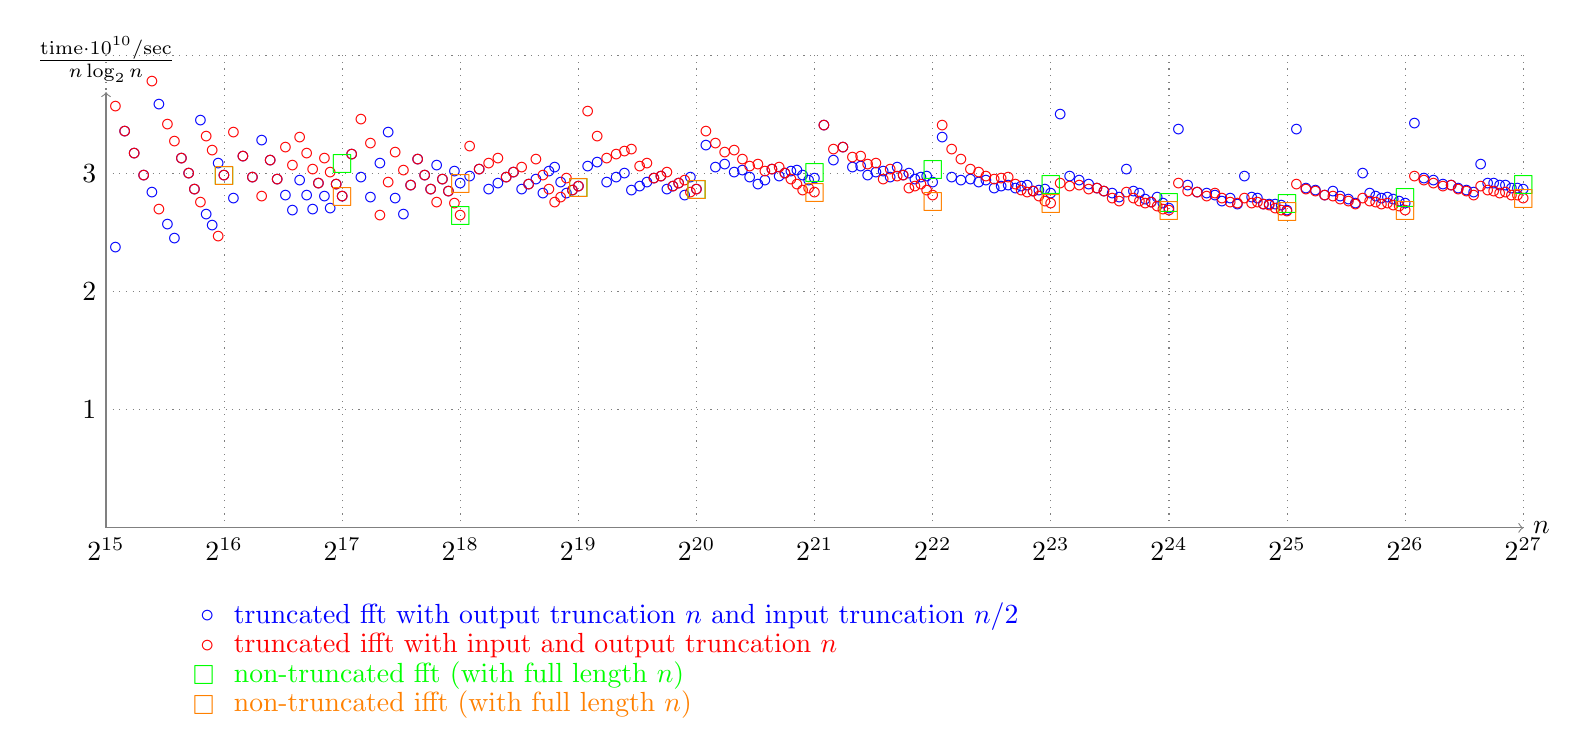
\begin{tikzpicture}[xscale=1.5, yscale=1.5]
\draw [dotted, gray] (15,0) grid (27,4);
\draw[latex-latex, thin, draw=gray, -to] (15,0)--(27,0) node [right] {$n$};
\draw[latex-latex, thin, draw=gray, -to] (15,0)--(15,3.69) node [above] {$\frac{\text{time} \cdot 10^{10}/\text{sec}}{n \log_2 n}$};

\foreach \Point in {1,2,3}{
    \node [black] at (15,\Point) [left] {$\Point$};
}

\foreach \Point in {15,16,...,27}{
    \node [black] at (\Point,0) [below] {$2^{\Point}$};
}

\foreach \Point in {(15.08,  2.37), (15.16,  3.35), (15.24,  3.16), (15.32,  2.98), (15.39,  2.83), (15.45,  3.58), (15.52,  2.56), (15.58,  2.44), (15.64,  3.12), (15.70,  2.99), (15.75,  2.86), (15.80,  3.44), (15.85,  2.65), (15.90,  2.55), (15.95,  3.08), (16.00,  2.98), (16.08,  2.78), (16.16,  3.14), (16.24,  2.96), (16.32,  3.27), (16.39,  3.10), (16.45,  2.94), (16.52,  2.81), (16.58,  2.68), (16.64,  2.93), (16.70,  2.81), (16.75,  2.69), (16.80,  2.91), (16.85,  2.80), (16.90,  2.70), (16.95,  2.90), (17.00,  2.80), (17.08,  3.15), (17.16,  2.96), (17.24,  2.79), (17.32,  3.08), (17.39,  3.34), (17.45,  2.78), (17.52,  2.65), (17.58,  2.89), (17.64,  3.11), (17.70,  2.98), (17.75,  2.86), (17.80,  3.06), (17.85,  2.94), (17.90,  2.84), (17.95,  3.01), (18.00,  2.91), (18.08,  2.97), (18.16,  3.03), (18.24,  2.86), (18.32,  2.91), (18.39,  2.96), (18.45,  3.00), (18.52,  2.86), (18.58,  2.90), (18.64,  2.94), (18.70,  2.82), (18.75,  3.01), (18.80,  3.04), (18.85,  2.92), (18.90,  2.82), (18.95,  2.85), (19.00,  2.88), (19.08,  3.05), (19.16,  3.09), (19.24,  2.92), (19.32,  2.96), (19.39,  2.99), (19.45,  2.85), (19.52,  2.88), (19.58,  2.92), (19.64,  2.95), (19.70,  2.97), (19.75,  2.86), (19.80,  2.88), (19.85,  2.91), (19.90,  2.81), (19.95,  2.96), (20.00,  2.86), (20.08,  3.23), (20.16,  3.04), (20.24,  3.07), (20.32,  3.00), (20.39,  3.02), (20.45,  2.96), (20.52,  2.90), (20.58,  2.93), (20.64,  3.03), (20.70,  2.97), (20.75,  2.99), (20.80,  3.01), (20.85,  3.02), (20.90,  2.98), (20.95,  2.93), (21.00,  2.95), (21.08,  3.40), (21.16,  3.10), (21.24,  3.21), (21.32,  3.04), (21.39,  3.05), (21.45,  2.98), (21.52,  3.00), (21.58,  3.01), (21.64,  2.96), (21.70,  3.04), (21.75,  2.98), (21.80,  2.99), (21.85,  2.94), (21.90,  2.96), (21.95,  2.97), (22.00,  2.92), (22.08,  3.30), (22.16,  2.96), (22.24,  2.93), (22.32,  2.94), (22.39,  2.92), (22.45,  2.93), (22.52,  2.87), (22.58,  2.88), (22.64,  2.89), (22.70,  2.87), (22.75,  2.88), (22.80,  2.89), (22.85,  2.84), (22.90,  2.85), (22.95,  2.86), (23.00,  2.82), (23.08,  3.49), (23.16,  2.97), (23.24,  2.93), (23.32,  2.90), (23.39,  2.87), (23.45,  2.84), (23.52,  2.82), (23.58,  2.79), (23.64,  3.03), (23.70,  2.84), (23.75,  2.82), (23.80,  2.77), (23.85,  2.75), (23.90,  2.79), (23.95,  2.74), (24.00,  2.70), (24.08,  3.37), (24.16,  2.89), (24.24,  2.83), (24.32,  2.82), (24.39,  2.81), (24.45,  2.76), (24.52,  2.78), (24.58,  2.73), (24.64,  2.97), (24.70,  2.79), (24.75,  2.78), (24.80,  2.73), (24.85,  2.73), (24.90,  2.73), (24.95,  2.72), (25.00,  2.68), (25.08,  3.37), (25.16,  2.87), (25.24,  2.85), (25.32,  2.81), (25.39,  2.84), (25.45,  2.80), (25.52,  2.77), (25.58,  2.74), (25.64,  2.99), (25.70,  2.82), (25.75,  2.80), (25.80,  2.78), (25.85,  2.79), (25.90,  2.77), (25.95,  2.76), (26.00,  2.74), (26.08,  3.42), (26.16,  2.95), (26.24,  2.93), (26.32,  2.90), (26.39,  2.89), (26.45,  2.87), (26.52,  2.85), (26.58,  2.83), (26.64,  3.07), (26.70,  2.91), (26.75,  2.91), (26.80,  2.89), (26.85,  2.89), (26.90,  2.87), (26.95,  2.87), (27.00,  2.86)}{
    \node [blue] at \Point {$\circ$};
}

\foreach \Point in {(15.08,  3.56), (15.16,  3.35), (15.24,  3.16), (15.32,  2.98), (15.39,  3.77), (15.45,  2.69), (15.52,  3.41), (15.58,  3.26), (15.64,  3.12), (15.70,  2.99), (15.75,  2.86), (15.80,  2.75), (15.85,  3.31), (15.90,  3.19), (15.95,  2.46), (16.00,  2.98), (16.08,  3.34), (16.16,  3.14), (16.24,  2.96), (16.32,  2.80), (16.39,  3.10), (16.45,  2.94), (16.52,  3.21), (16.58,  3.06), (16.64,  3.30), (16.70,  3.16), (16.75,  3.03), (16.80,  2.91), (16.85,  3.12), (16.90,  3.00), (16.95,  2.90), (17.00,  2.80), (17.08,  3.15), (17.16,  3.45), (17.24,  3.25), (17.32,  2.64), (17.39,  2.92), (17.45,  3.17), (17.52,  3.02), (17.58,  2.89), (17.64,  3.11), (17.70,  2.98), (17.75,  2.86), (17.80,  2.75), (17.85,  2.94), (17.90,  2.84), (17.95,  2.74), (18.00,  2.64), (18.08,  3.22), (18.16,  3.03), (18.24,  3.08), (18.32,  3.12), (18.39,  2.96), (18.45,  3.00), (18.52,  3.04), (18.58,  2.90), (18.64,  3.11), (18.70,  2.98), (18.75,  2.86), (18.80,  2.75), (18.85,  2.79), (18.90,  2.95), (18.95,  2.85), (19.00,  2.88), (19.08,  3.52), (19.16,  3.31), (19.24,  3.12), (19.32,  3.15), (19.39,  3.18), (19.45,  3.20), (19.52,  3.05), (19.58,  3.08), (19.64,  2.95), (19.70,  2.97), (19.75,  3.00), (19.80,  2.88), (19.85,  2.91), (19.90,  2.93), (19.95,  2.83), (20.00,  2.86), (20.08,  3.35), (20.16,  3.25), (20.24,  3.17), (20.32,  3.19), (20.39,  3.11), (20.45,  3.05), (20.52,  3.07), (20.58,  3.01), (20.64,  3.03), (20.70,  3.04), (20.75,  2.99), (20.80,  2.94), (20.85,  2.90), (20.90,  2.85), (20.95,  2.87), (21.00,  2.83), (21.08,  3.40), (21.16,  3.20), (21.24,  3.21), (21.32,  3.13), (21.39,  3.14), (21.45,  3.07), (21.52,  3.08), (21.58,  2.94), (21.64,  3.03), (21.70,  2.97), (21.75,  2.98), (21.80,  2.87), (21.85,  2.88), (21.90,  2.90), (21.95,  2.85), (22.00,  2.81), (22.08,  3.40), (22.16,  3.20), (22.24,  3.11), (22.32,  3.03), (22.39,  3.00), (22.45,  2.97), (22.52,  2.94), (22.58,  2.95), (22.64,  2.96), (22.70,  2.90), (22.75,  2.85), (22.80,  2.83), (22.85,  2.84), (22.90,  2.80), (22.95,  2.76), (23.00,  2.74), (23.08,  2.91), (23.16,  2.88), (23.24,  2.89), (23.32,  2.86), (23.39,  2.87), (23.45,  2.84), (23.52,  2.78), (23.58,  2.76), (23.64,  2.83), (23.70,  2.78), (23.75,  2.76), (23.80,  2.74), (23.85,  2.75), (23.90,  2.71), (23.95,  2.69), (24.00,  2.68), (24.08,  2.91), (24.16,  2.84), (24.24,  2.83), (24.32,  2.80), (24.39,  2.82), (24.45,  2.78), (24.52,  2.75), (24.58,  2.74), (24.64,  2.78), (24.70,  2.74), (24.75,  2.75), (24.80,  2.73), (24.85,  2.72), (24.90,  2.70), (24.95,  2.68), (25.00,  2.67), (25.08,  2.90), (25.16,  2.86), (25.24,  2.84), (25.32,  2.81), (25.39,  2.80), (25.45,  2.77), (25.52,  2.76), (25.58,  2.73), (25.64,  2.78), (25.70,  2.76), (25.75,  2.75), (25.80,  2.73), (25.85,  2.74), (25.90,  2.72), (25.95,  2.71), (26.00,  2.68), (26.08,  2.97), (26.16,  2.93), (26.24,  2.91), (26.32,  2.88), (26.39,  2.89), (26.45,  2.86), (26.52,  2.84), (26.58,  2.81), (26.64,  2.88), (26.70,  2.85), (26.75,  2.84), (26.80,  2.82), (26.85,  2.83), (26.90,  2.81), (26.95,  2.81), (27.00,  2.78)}{
    \node [red] at \Point {$\circ$};
}

\foreach \Point in {(16.00,  2.98), (17.00,  3.08), (18.00,  2.64), (19.00,  2.88), (20.00,  2.86), (21.00,  3.00), (22.00,  3.03), (23.00,  2.90), (24.00,  2.75), (25.00,  2.74), (26.00,  2.79), (27.00,  2.90)}{
    \node [green] at \Point {$\square$};
}

\foreach \Point in {(16.00,  2.98), (17.00,  2.80), (18.00,  2.91), (19.00,  2.88), (20.00,  2.86), (21.00,  2.83), (22.00,  2.76), (23.00,  2.74), (24.00,  2.68), (25.00,  2.67), (26.00,  2.68), (27.00,  2.78)}{
    \node [orange] at \Point {$\square$};
}


\node [blue] at (16,-0.75) [left] {$\circ$};
\node [blue] at (16,-0.75) [right] {truncated fft with output truncation $n$ and input truncation $n/2$};

\node [red] at (16,-1.0) [left] {$\circ$};
\node [red] at (16,-1.0) [right] {truncated ifft with input and output truncation $n$};

\node [green] at (16,-1.25) [left] {$\square$};
\node [green] at (16,-1.25) [right] {non-truncated fft (with full length $n$)};

\node [orange] at (16,-1.5) [left] {$\square$};
\node [orange] at (16,-1.5) [right] {non-truncated ifft (with full length $n$)};

\end{tikzpicture}
\end{figure}

\begin{figure}
\caption{Truncation effectiveness with $50$ bit coefficients and optimized length $16$ basecase}
\label{trunc2}
\centering
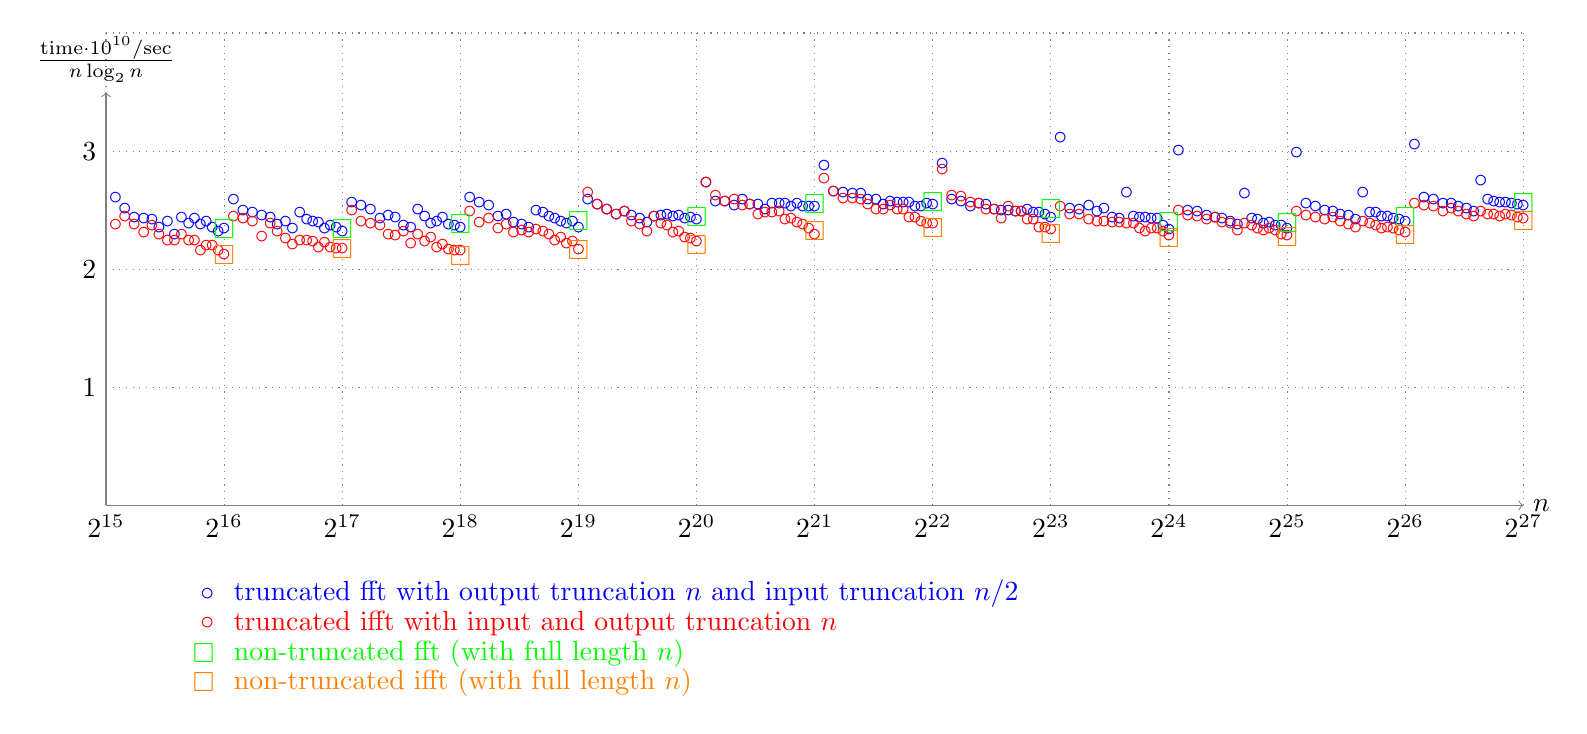
\begin{tikzpicture}[xscale=1.5, yscale=1.5]
\draw [dotted, gray] (15,0) grid (27,4);
\draw[latex-latex, thin, draw=gray, -to] (15,0)--(27,0) node [right] {$n$};
\draw[latex-latex, thin, draw=gray, -to] (15,0)--(15,3.5) node [above] {$\frac{\text{time} \cdot 10^{10}/\text{sec}}{n \log_2 n}$};

\foreach \Point in {1,2,3}{
    \node [black] at (15,\Point) [left] {$\Point$};
}

\foreach \Point in {15,16,...,27}{
    \node [black] at (\Point,0) [below] {$2^{\Point}$};
}

\foreach \Point in {(15.08,  2.60), (15.16,  2.51), (15.24,  2.43), (15.32,  2.42), (15.39,  2.41), (15.45,  2.35), (15.52,  2.40), (15.58,  2.29), (15.64,  2.43), (15.70,  2.38), (15.75,  2.42), (15.80,  2.37), (15.85,  2.40), (15.90,  2.35), (15.95,  2.31), (16.00,  2.34), (16.08,  2.58), (16.16,  2.49), (16.24,  2.47), (16.32,  2.45), (16.39,  2.43), (16.45,  2.37), (16.52,  2.40), (16.58,  2.34), (16.64,  2.47), (16.70,  2.41), (16.75,  2.40), (16.80,  2.39), (16.85,  2.34), (16.90,  2.36), (16.95,  2.35), (17.00,  2.31), (17.08,  2.56), (17.16,  2.53), (17.24,  2.50), (17.32,  2.42), (17.39,  2.45), (17.45,  2.43), (17.52,  2.36), (17.58,  2.35), (17.64,  2.50), (17.70,  2.44), (17.75,  2.38), (17.80,  2.40), (17.85,  2.43), (17.90,  2.37), (17.95,  2.36), (18.00,  2.35), (18.08,  2.60), (18.16,  2.56), (18.24,  2.53), (18.32,  2.44), (18.39,  2.46), (18.45,  2.39), (18.52,  2.37), (18.58,  2.35), (18.64,  2.49), (18.70,  2.47), (18.75,  2.44), (18.80,  2.42), (18.85,  2.40), (18.90,  2.38), (18.95,  2.40), (19.00,  2.35), (19.08,  2.58), (19.16,  2.54), (19.24,  2.50), (19.32,  2.46), (19.39,  2.48), (19.45,  2.45), (19.52,  2.42), (19.58,  2.39), (19.64,  2.44), (19.70,  2.45), (19.75,  2.46), (19.80,  2.44), (19.85,  2.45), (19.90,  2.42), (19.95,  2.43), (20.00,  2.41), (20.08,  2.73), (20.16,  2.57), (20.24,  2.57), (20.32,  2.53), (20.39,  2.58), (20.45,  2.54), (20.52,  2.54), (20.58,  2.50), (20.64,  2.55), (20.70,  2.55), (20.75,  2.55), (20.80,  2.52), (20.85,  2.55), (20.90,  2.52), (20.95,  2.52), (21.00,  2.52), (21.08,  2.87), (21.16,  2.65), (21.24,  2.64), (21.32,  2.63), (21.39,  2.63), (21.45,  2.58), (21.52,  2.58), (21.58,  2.54), (21.64,  2.57), (21.70,  2.56), (21.75,  2.56), (21.80,  2.56), (21.85,  2.52), (21.90,  2.52), (21.95,  2.55), (22.00,  2.54), (22.08,  2.89), (22.16,  2.58), (22.24,  2.57), (22.32,  2.52), (22.39,  2.55), (22.45,  2.54), (22.52,  2.50), (22.58,  2.49), (22.64,  2.49), (22.70,  2.48), (22.75,  2.48), (22.80,  2.50), (22.85,  2.47), (22.90,  2.47), (22.95,  2.46), (23.00,  2.43), (23.08,  3.11), (23.16,  2.51), (23.24,  2.50), (23.32,  2.53), (23.39,  2.48), (23.45,  2.51), (23.52,  2.43), (23.58,  2.42), (23.64,  2.64), (23.70,  2.44), (23.75,  2.43), (23.80,  2.43), (23.85,  2.42), (23.90,  2.42), (23.95,  2.36), (24.00,  2.33), (24.08,  3.00), (24.16,  2.49), (24.24,  2.48), (24.32,  2.45), (24.39,  2.43), (24.45,  2.42), (24.52,  2.40), (24.58,  2.37), (24.64,  2.63), (24.70,  2.42), (24.75,  2.41), (24.80,  2.38), (24.85,  2.39), (24.90,  2.36), (24.95,  2.36), (25.00,  2.34), (25.08,  2.98), (25.16,  2.55), (25.24,  2.52), (25.32,  2.49), (25.39,  2.48), (25.45,  2.46), (25.52,  2.45), (25.58,  2.41), (25.64,  2.64), (25.70,  2.47), (25.75,  2.47), (25.80,  2.44), (25.85,  2.44), (25.90,  2.42), (25.95,  2.41), (26.00,  2.40), (26.08,  3.05), (26.16,  2.60), (26.24,  2.58), (26.32,  2.55), (26.39,  2.55), (26.45,  2.52), (26.52,  2.51), (26.58,  2.48), (26.64,  2.74), (26.70,  2.58), (26.75,  2.57), (26.80,  2.56), (26.85,  2.56), (26.90,  2.55), (26.95,  2.54), (27.00,  2.53)}{
    \node [blue] at \Point {$\circ$};
}

\foreach \Point in {(15.08,  2.37), (15.16,  2.44), (15.24,  2.37), (15.32,  2.30), (15.39,  2.36), (15.45,  2.29), (15.52,  2.24), (15.58,  2.24), (15.64,  2.29), (15.70,  2.24), (15.75,  2.24), (15.80,  2.15), (15.85,  2.19), (15.90,  2.19), (15.95,  2.15), (16.00,  2.12), (16.08,  2.44), (16.16,  2.42), (16.24,  2.40), (16.32,  2.27), (16.39,  2.38), (16.45,  2.31), (16.52,  2.25), (16.58,  2.20), (16.64,  2.24), (16.70,  2.24), (16.75,  2.23), (16.80,  2.18), (16.85,  2.22), (16.90,  2.18), (16.95,  2.17), (17.00,  2.17), (17.08,  2.49), (17.16,  2.40), (17.24,  2.38), (17.32,  2.36), (17.39,  2.29), (17.45,  2.28), (17.52,  2.31), (17.58,  2.21), (17.64,  2.29), (17.70,  2.23), (17.75,  2.26), (17.80,  2.18), (17.85,  2.20), (17.90,  2.16), (17.95,  2.15), (18.00,  2.15), (18.08,  2.48), (18.16,  2.39), (18.24,  2.42), (18.32,  2.34), (18.39,  2.37), (18.45,  2.30), (18.52,  2.32), (18.58,  2.30), (18.64,  2.33), (18.70,  2.31), (18.75,  2.29), (18.80,  2.24), (18.85,  2.26), (18.90,  2.21), (18.95,  2.23), (19.00,  2.16), (19.08,  2.64), (19.16,  2.54), (19.24,  2.50), (19.32,  2.46), (19.39,  2.48), (19.45,  2.40), (19.52,  2.37), (19.58,  2.31), (19.64,  2.44), (19.70,  2.38), (19.75,  2.36), (19.80,  2.30), (19.85,  2.31), (19.90,  2.26), (19.95,  2.25), (20.00,  2.23), (20.08,  2.73), (20.16,  2.62), (20.24,  2.57), (20.32,  2.58), (20.39,  2.53), (20.45,  2.54), (20.52,  2.46), (20.58,  2.47), (20.64,  2.47), (20.70,  2.48), (20.75,  2.41), (20.80,  2.42), (20.85,  2.39), (20.90,  2.37), (20.95,  2.34), (21.00,  2.29), (21.08,  2.76), (21.16,  2.65), (21.24,  2.59), (21.32,  2.59), (21.39,  2.58), (21.45,  2.54), (21.52,  2.50), (21.58,  2.50), (21.64,  2.53), (21.70,  2.50), (21.75,  2.50), (21.80,  2.43), (21.85,  2.43), (21.90,  2.40), (21.95,  2.38), (22.00,  2.38), (22.08,  2.84), (22.16,  2.62), (22.24,  2.61), (22.32,  2.56), (22.39,  2.55), (22.45,  2.50), (22.52,  2.50), (22.58,  2.42), (22.64,  2.52), (22.70,  2.48), (22.75,  2.48), (22.80,  2.41), (22.85,  2.41), (22.90,  2.35), (22.95,  2.35), (23.00,  2.33), (23.08,  2.52), (23.16,  2.46), (23.24,  2.46), (23.32,  2.41), (23.39,  2.40), (23.45,  2.40), (23.52,  2.39), (23.58,  2.39), (23.64,  2.38), (23.70,  2.38), (23.75,  2.34), (23.80,  2.31), (23.85,  2.34), (23.90,  2.34), (23.95,  2.31), (24.00,  2.28), (24.08,  2.49), (24.16,  2.45), (24.24,  2.44), (24.32,  2.41), (24.39,  2.43), (24.45,  2.39), (24.52,  2.38), (24.58,  2.32), (24.64,  2.38), (24.70,  2.36), (24.75,  2.34), (24.80,  2.32), (24.85,  2.34), (24.90,  2.32), (24.95,  2.29), (25.00,  2.28), (25.08,  2.48), (25.16,  2.45), (25.24,  2.43), (25.32,  2.41), (25.39,  2.43), (25.45,  2.40), (25.52,  2.37), (25.58,  2.35), (25.64,  2.40), (25.70,  2.38), (25.75,  2.36), (25.80,  2.34), (25.85,  2.35), (25.90,  2.34), (25.95,  2.32), (26.00,  2.30), (26.08,  2.55), (26.16,  2.53), (26.24,  2.52), (26.32,  2.48), (26.39,  2.51), (26.45,  2.48), (26.52,  2.46), (26.58,  2.44), (26.64,  2.48), (26.70,  2.46), (26.75,  2.46), (26.80,  2.44), (26.85,  2.46), (26.90,  2.45), (26.95,  2.43), (27.00,  2.42)}{
    \node [red] at \Point {$\circ$};
}

\foreach \Point in {(16.00,  2.34), (17.00,  2.34), (18.00,  2.38), (19.00,  2.41), (20.00,  2.44), (21.00,  2.55), (22.00,  2.57), (23.00,  2.51), (24.00,  2.40), (25.00,  2.39), (26.00,  2.44), (27.00,  2.56)}{
    \node [green] at \Point {$\square$};
}

\foreach \Point in {(16.00,  2.12), (17.00,  2.17), (18.00,  2.11), (19.00,  2.16), (20.00,  2.20), (21.00,  2.32), (22.00,  2.35), (23.00,  2.30), (24.00,  2.26), (25.00,  2.27), (26.00,  2.29), (27.00,  2.41)}{
    \node [orange] at \Point {$\square$};
}


\node [blue] at (16,-0.75) [left] {$\circ$};
\node [blue] at (16,-0.75) [right] {truncated fft with output truncation $n$ and input truncation $n/2$};

\node [red] at (16,-1.0) [left] {$\circ$};
\node [red] at (16,-1.0) [right] {truncated ifft with input and output truncation $n$};

\node [green] at (16,-1.25) [left] {$\square$};
\node [green] at (16,-1.25) [right] {non-truncated fft (with full length $n$)};

\node [orange] at (16,-1.5) [left] {$\square$};
\node [orange] at (16,-1.5) [right] {non-truncated ifft (with full length $n$)};

\end{tikzpicture}
\end{figure}

\begin{figure}
\caption{Truncation effectiveness of \texttt{\{i\}fft\_mfa\_truncate\_sqrt2} with $2^{16}$ bit coefficients}
\label{trunc_flint}
\centering
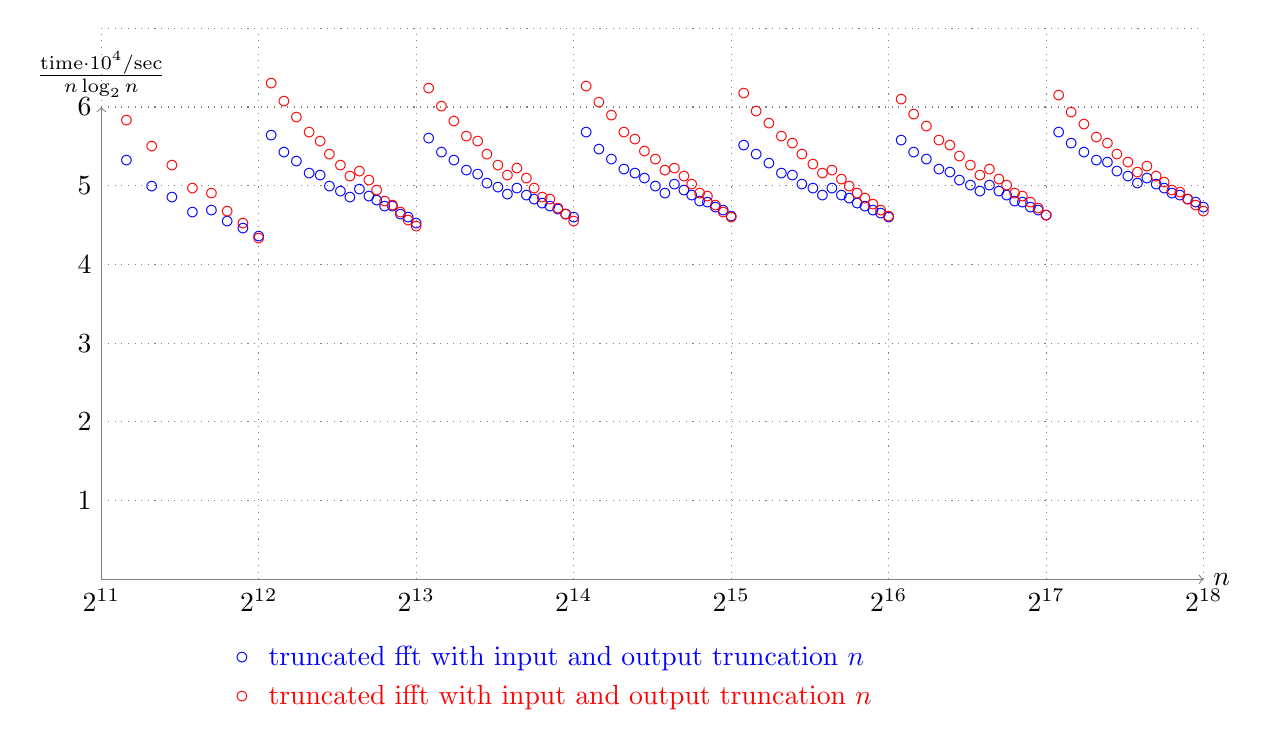
\begin{tikzpicture}[xscale=2.0, yscale=1.0]
\draw [dotted, gray] (11,0) grid (18,7);
\draw[latex-latex, thin, draw=gray, -to] (11,0)--(18,0) node [right] {$n$};
\draw[latex-latex, thin, draw=gray, -to] (11,0)--(11,6) node [above] {$\frac{\text{time} \cdot 10^{4}/\text{sec}}{n \log_2 n}$};

\foreach \Point in {1,2,3,4,5,6}{
    \node [black] at (11,\Point) [left] {$\Point$};
}

\foreach \Point in {11,12,...,18}{
    \node [black] at (\Point,0) [below] {$2^{\Point}$};
}

\foreach \Point in {(11.16,  5.31), (11.32,  4.98), (11.45,  4.84), (11.58,  4.65), (11.70,  4.67), (11.80,  4.54), (11.90,  4.44), (12.00,  4.34), (12.08,  5.63), (12.16,  5.41), (12.24,  5.30), (12.32,  5.15), (12.39,  5.12), (12.45,  4.98), (12.52,  4.91), (12.58,  4.84), (12.64,  4.94), (12.70,  4.85), (12.75,  4.80), (12.80,  4.73), (12.85,  4.72), (12.90,  4.62), (12.95,  4.58), (13.00,  4.51), (13.08,  5.59), (13.16,  5.41), (13.24,  5.31), (13.32,  5.18), (13.39,  5.13), (13.45,  5.02), (13.52,  4.97), (13.58,  4.88), (13.64,  4.96), (13.70,  4.87), (13.75,  4.82), (13.80,  4.76), (13.85,  4.73), (13.90,  4.69), (13.95,  4.62), (14.00,  4.58), (14.08,  5.66), (14.16,  5.45), (14.24,  5.32), (14.32,  5.19), (14.39,  5.15), (14.45,  5.08), (14.52,  4.98), (14.58,  4.89), (14.64,  5.01), (14.70,  4.93), (14.75,  4.86), (14.80,  4.79), (14.85,  4.78), (14.90,  4.71), (14.95,  4.67), (15.00,  4.60), (15.08,  5.50), (15.16,  5.38), (15.24,  5.27), (15.32,  5.14), (15.39,  5.12), (15.45,  5.01), (15.52,  4.96), (15.58,  4.86), (15.64,  4.96), (15.70,  4.86), (15.75,  4.83), (15.80,  4.76), (15.85,  4.73), (15.90,  4.67), (15.95,  4.64), (16.00,  4.58), (16.08,  5.56), (16.16,  5.41), (16.24,  5.32), (16.32,  5.20), (16.39,  5.16), (16.45,  5.05), (16.52,  4.99), (16.58,  4.91), (16.64,  4.99), (16.70,  4.92), (16.75,  4.86), (16.80,  4.79), (16.85,  4.77), (16.90,  4.71), (16.95,  4.67), (17.00,  4.61), (17.08,  5.66), (17.16,  5.52), (17.24,  5.41), (17.32,  5.31), (17.39,  5.28), (17.45,  5.17), (17.52,  5.10), (17.58,  5.02), (17.64,  5.08), (17.70,  5.01), (17.75,  4.95), (17.80,  4.89), (17.85,  4.87), (17.90,  4.81), (17.95,  4.77), (18.00,  4.71)}{
    \node [blue] at \Point {$\circ$};
}

\foreach \Point in {(11.16,  5.82), (11.32,  5.49), (11.45,  5.24), (11.58,  4.95), (11.70,  4.89), (11.80,  4.66), (11.90,  4.51), (12.00,  4.32), (12.08,  6.29), (12.16,  6.06), (12.24,  5.85), (12.32,  5.66), (12.39,  5.55), (12.45,  5.39), (12.52,  5.25), (12.58,  5.10), (12.64,  5.17), (12.70,  5.05), (12.75,  4.93), (12.80,  4.79), (12.85,  4.74), (12.90,  4.65), (12.95,  4.55), (13.00,  4.47), (13.08,  6.23), (13.16,  5.99), (13.24,  5.81), (13.32,  5.62), (13.39,  5.55), (13.45,  5.39), (13.52,  5.25), (13.58,  5.12), (13.64,  5.21), (13.70,  5.08), (13.75,  4.96), (13.80,  4.84), (13.85,  4.81), (13.90,  4.70), (13.95,  4.62), (14.00,  4.54), (14.08,  6.25), (14.16,  6.04), (14.24,  5.88), (14.32,  5.67), (14.39,  5.58), (14.45,  5.43), (14.52,  5.32), (14.58,  5.18), (14.64,  5.21), (14.70,  5.11), (14.75,  5.01), (14.80,  4.89), (14.85,  4.85), (14.90,  4.74), (14.95,  4.65), (15.00,  4.59), (15.08,  6.16), (15.16,  5.93), (15.24,  5.78), (15.32,  5.62), (15.39,  5.52), (15.45,  5.38), (15.52,  5.26), (15.58,  5.15), (15.64,  5.18), (15.70,  5.07), (15.75,  4.98), (15.80,  4.89), (15.85,  4.83), (15.90,  4.75), (15.95,  4.67), (16.00,  4.60), (16.08,  6.09), (16.16,  5.89), (16.24,  5.74), (16.32,  5.56), (16.39,  5.50), (16.45,  5.36), (16.52,  5.25), (16.58,  5.12), (16.64,  5.19), (16.70,  5.07), (16.75,  4.99), (16.80,  4.89), (16.85,  4.85), (16.90,  4.77), (16.95,  4.70), (17.00,  4.61), (17.08,  6.13), (17.16,  5.92), (17.24,  5.77), (17.32,  5.60), (17.39,  5.52), (17.45,  5.38), (17.52,  5.28), (17.58,  5.16), (17.64,  5.23), (17.70,  5.11), (17.75,  5.03), (17.80,  4.93), (17.85,  4.90), (17.90,  4.81), (17.95,  4.74), (18.00,  4.66)}{
    \node [red] at \Point {$\circ$};
}


\node [blue] at (12,-1.0) [left] {$\circ$};
\node [blue] at (12,-1.0) [right] {truncated fft with input and output truncation $n$};

\node [red] at (12,-1.5) [left] {$\circ$};
\node [red] at (12,-1.5) [right] {truncated ifft with input and output truncation $n$};


\end{tikzpicture}
\end{figure}




\end{document}

